\documentclass[12pt]{article}
\usepackage[a4paper, margin=1in]{geometry}
\usepackage{setspace}
\usepackage{graphicx}
\usepackage{enumitem}

\onehalfspacing

\title{Taboo Language Classification and Analysis in Sinhala Text Data}
\author{}
\date{}

\begin{document}

\maketitle

\section{Introduction}

Sinhala is a low-resource language primarily spoken in Sri Lanka, with limited availability of annotated datasets and Natural Language Processing (NLP) tools. Compared to widely studied languages such as English, research on offensive language detection in Sinhala remains relatively underdeveloped. This creates challenges in identifying and analyzing taboo or harmful expressions, especially in informal digital communication such as social media. Furthermore, Sinhala offensive language is often context-dependent and may involve cultural nuances, making classification more complex. Therefore, this component of the project focuses specifically on the identification, categorization, and analysis of Sinhala taboo language, contributing toward improving NLP resources and understanding of offensive language in low-resource linguistic settings.

\section{Objectives}

The primary goal of this project is to systematically analyze offensive Sinhala language data. The specific objectives are as follows:

\begin{itemize}
    \item To collect and organize a dataset of Sinhala taboo and offensive words
    \item To classify offensive terms into meaningful semantic categories such as Gender, politics, disability-related, and race-related expressions
    \item To design and implement a target-type classification framework to identify whether offensive language is directed toward:
    \begin{itemize}
        \item Individuals (IND)
        \item Groups (GRP)
        \item Untargeted entities (UNT)
    \end{itemize}
    \item To perform exploratory data analysis (EDA) to uncover patterns and trends in offensive language usage
    \item To visualize key findings using appropriate graphical representations
    \item To identify challenges associated with processing and analyzing Sinhala text data
\end{itemize}

\section{Dataset Description}

The dataset used in this project consists of a curated collection of Sinhala offensive words along with their associated metadata. The dataset is structured in a tabular format and includes the following attributes:

\subsection{Attributes in the Original Dataset}

\begin{itemize}
    \item post\_id: A unique identifier assigned to each entry
    \item text: The offensive or taboo term in Sinhala
    \item tokens: Tokenized text
    \item label: OFF - offensive or NOT – not offensive
    \item rationales: text annotation data (0 – non offensive and 1- offensive)
\end{itemize}

\subsection{Attributes Derived from the Original Dataset}

\begin{itemize}
    \item category: The type of offensiveness - Gender, Politics, Race, Religion , Citizenship , Age , Disability , National Origin

    Initial Manual annotation and based on that data used AI models to update the category.

    \item off\_word\_count: Number of taboo/ offensive words per record

    \item offensive words: List of Taboo/ Offensive words per record
\end{itemize}

\subsection{Derived Data Based on Rationales Column}

\begin{itemize}
    \item target type: To enhance the analytical value of the dataset, an additional column named target\_type was introduced. This column categorizes offensive language based on its intended target:

    \begin{itemize}
        \item IND (Individual): Offensive language directed at a specific person
        \item GRP (Group): Language targeting a group defined by shared characteristics (e.g., gender, race)
        \item UNT (Untargeted): General offensive expressions without a specific target
    \end{itemize}

    Used 2 separate manually annotated IND and GRP list of dataset to update the columns.
\end{itemize}

\subsection{Multi-Category Entries}

A notable characteristic of the dataset is that some entries belong to multiple categories. For example: ``Disability, Gender''

Such cases reflect the overlapping nature of offensive language, where a single term may simultaneously target multiple social dimensions. Handling these entries required additional preprocessing steps to ensure accurate analysis.

\begin{figure}[h]
\centering
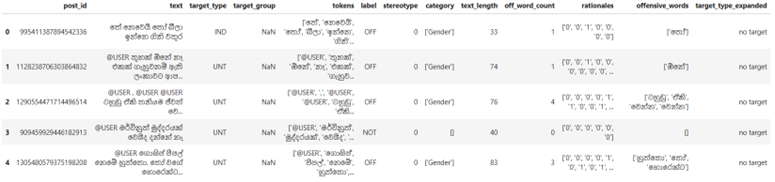
\includegraphics[width=0.8\textwidth]{figure1.png}
\caption{Sample Structure of the Dataset}
\end{figure}

\section{Data Preprocessing}

Data preprocessing is a crucial step in ensuring the quality and reliability of analysis. Several preprocessing techniques were applied to the dataset.

\subsection{Data Cleaning}

\begin{itemize}
    \item Removal of unwanted characters and extra spaces
    \item Standardization of text formatting
    \item Creation of new derived columns
    \item Extraction of offensive words from rationales
    \item Assignment of target types
\end{itemize}

\subsection{Handling Multi-Label Categories}

Multi-category entries were split into separate rows to enable proper analysis.

This process:
\begin{itemize}
    \item Convert category strings into lists
    \item Expands each category into a separate row
    \item Enables accurate frequency analysis of individual categories
\end{itemize}

\subsection{Encoding and Font Handling}

Since the dataset contains Sinhala characters, special attention was given to encoding and visualization:

\begin{itemize}
    \item UTF-8 encoding was ensured throughout the dataset
    \item Font issues in visualization libraries were handled to correctly display Sinhala text
\end{itemize}

\subsection{Target-Type Assignment}

A rule-based approach was used to assign values to the target\_type column. This involved analyzing the meaning and usage context of each word and mapping it to the appropriate target category.

\section{Methodology}

\subsection{Classification Strategy}

\begin{itemize}
    \item Offensive words were categorized based on predefined semantic labels
    \item Target types were assigned using linguistic interpretation and contextual understanding
\end{itemize}

\subsection{Frequency Analysis}

Frequency distributions were computed to understand patterns in offensive language usage.

This operation:
\begin{itemize}
    \item Counts the number of occurrences of offensive word counts
    \item Sorts the results in ascending order
    \item Helps identify common and rare patterns in the dataset
\end{itemize}

\subsection{Analytical Approach}

The analysis focused on:
\begin{itemize}
    \item Category frequency distribution
    \item Target-type distribution
    \item Co-occurrence of multiple categories
\end{itemize}

\section{Data Analysis and Visualization}

Exploratory Data Analysis (EDA) was performed to extract meaningful insights.

\subsection{Category Distribution Analysis}

The frequency of each category was computed to identify dominant types of offensive language. The use multi category and exploded as two approaches.

As shown in Figure 2 gender-related offensive language appears as the most dominant category in the dataset. This indicates that insults targeting gender are significantly more prevalent compared to other categories such as disability and age. Furthermore, the presence of multi-category entries highlights the intersectionality of offensive language, where a single expression may simultaneously target multiple social dimensions.

\begin{figure}[h]
\centering
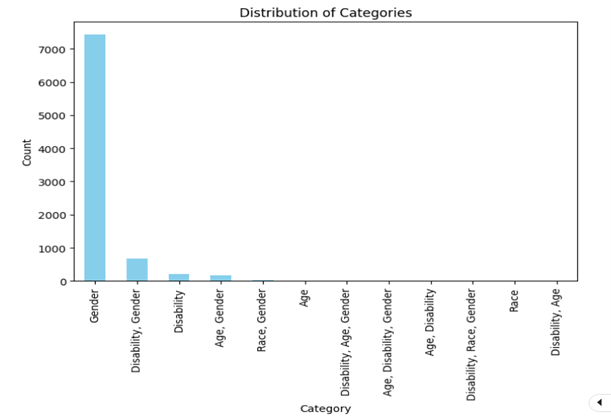
\includegraphics[width=0.8\textwidth]{figure2.png}
\caption{Distribution of offensive language categories (multiple), showing gender as the most frequent category}
\end{figure}

\begin{figure}[h]
\centering
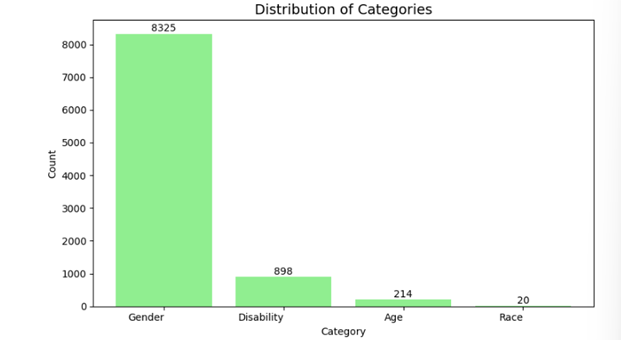
\includegraphics[width=0.8\textwidth]{figure3.png}
\caption{Distribution of offensive language categories, showing gender as the most frequent category}
\end{figure}

\subsection{Target-Type Distribution}

The distribution of target types (IND, GRP, UNT) was analyzed to understand how offensive language is directed. This provides insight into whether offensive expressions are more personalized or generalized.

Figure 4 illustrates that the majority of offensive expressions are directed toward individuals (IND). In contrast, lowest instances are categorized as untargeted (GRP). This suggests that offensive language is predominantly used in a targeted manner, focusing on specific individuals.

\subsection{Offensive Word Count Distribution}

\begin{figure}[h]
\centering
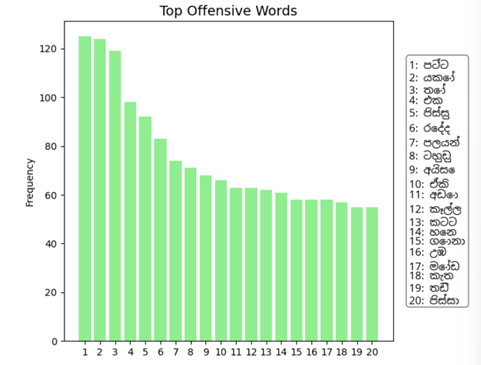
\includegraphics[width=0.8\textwidth]{figure6.png}
\caption{Histogram showing the distribution of offensive word counts per entry}
\end{figure}

Histograms were used to analyze the number of offensive words per entry.

As shown in Figure 5, the distribution of offensive words reveals that most entries contain a small number of offensive words. The frequency decreases as the number of words increases, indicating that offensive expressions are typically short and concise rather than extended phrases. This pattern reflects the nature of informal communication, where brief expressions are commonly used.

\subsection{Most Frequent Offensive Words}

\begin{figure}[h]
\centering
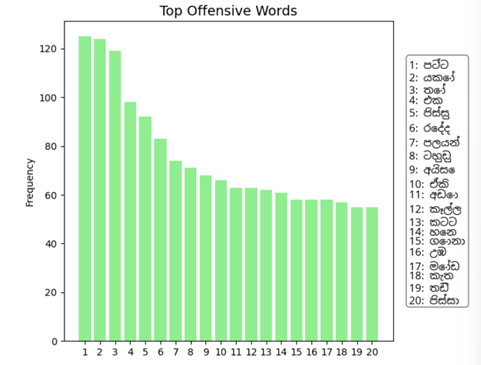
\includegraphics[width=0.8\textwidth]{figure7.png}
\caption{Most Frequent offensive words}
\end{figure}

\section{Results and Findings}

The analysis produced several important findings:

\begin{itemize}
    \item Gender-related offensive language was the most frequent category, indicating a strong presence of gender-based insults
    \item A significant number of entries contained multiple categories, highlighting overlapping forms of discrimination
    \item The majority of offensive expressions were directed toward individuals (IND)
\end{itemize}

These findings demonstrate that offensive language is complex, multi-dimensional, and often context dependent.

\section{Challenges}

Several challenges were encountered during the project:

\begin{itemize}
    \item Ambiguity in classification: Some words could belong to multiple categories depending on context
    \item Limited resources: Lack of existing Sinhala NLP tools and annotated datasets
    \item Data complexity: Multi-label entries required additional processing
    \item Technical issues: Encoding and font rendering problems during visualization
\end{itemize}

\section{Conclusion}

This study presented a structured analysis of Sinhala offensive language by developing a categorized dataset and applying a target-type classification framework. The findings reveal that offensive language in Sinhala is highly concentrated around gender-related expressions and is often directed toward individuals in nature.

The analysis also highlights the complexity of offensive language, as many expressions span multiple categories and depend heavily on context. Additionally, the presence of class imbalance in the dataset indicates potential challenges for building robust and unbiased machine learning models.

Overall, this work contributes to addressing the gap in Sinhala NLP resources by providing a foundation for future research in offensive language detection. Further improvements can be achieved by expanding the dataset, incorporating contextual understanding, and developing more advanced classification approaches.

\section{References}
\bibliography{refernce}

\begin{itemize}
    \item SOLD: Sinhala Offensive Language Dataset
    \item Jayaweera, L., \& Seneviratne, H. (2019). Challenges in Sinhala NLP: Tokenization and Morphological Analysis
\end{itemize}

\section{Appendix}

\subsection{OFF vs NOT Word Count Histogram}

This histogram illustrates the distribution of text entries based on their word counts, separated by offensive (OFF) and non-offensive (NOT) labels. The visualization shows that most entries, regardless of class, contain a relatively small number of words. Additionally, the overlap between OFF and NOT distributions suggests that text length alone is not a strong indicator of offensiveness, highlighting the importance of contextual and semantic analysis.

\subsection{Similarity of Target Group Attributes Based on Hate Spans}

This scatter plot represents the semantic relationships between different target group categories derived from hate span analysis. Each point corresponds to a category or combination of categories (e.g., Gender, Disability, Age), positioned in a two-dimensional semantic space.

The proximity between points indicates similarity in how these categories are targeted in offensive language. The size of each point reflects the relative frequency of occurrences. Notably, gender-related categories appear more prominent and frequently clustered with other attributes, suggesting that gender is often combined with other forms of offensive targeting such as disability or age.

\subsection{Category Distribution}

This figure presents the normalized distribution of offensive language categories within the dataset. The results indicate a significant class imbalance, with the Gender category dominating the dataset (approximately 87\%). Other categories such as Disability, Age, and Race appear with much lower frequencies, often in combination with Gender.

This imbalance highlights a key limitation of the dataset, as models trained on such data may become biased toward the majority class. It also reflects real-world trends where gender-based offensive language is more prevalent in the collected data.

\end{document}
